\documentclass[twoside,10pt]{article}

%================================ PREAMBLE ==================================

%--------- Packages -----------
\usepackage{fullpage}
\usepackage{amssymb}
\usepackage{amsmath}
\usepackage{amsthm}
\usepackage{latexsym}
\usepackage{graphicx}
\usepackage{color}
\usepackage{url}
\usepackage{listings}
\usepackage{pdfpages}
\usepackage{epstopdf}

%\usepackage{algorithm,algorithmic}

%----------Spacing-------------
%\setlength{\oddsidemargin}{0.25 in}
%\setlength{\evensidemargin}{-0.25 in}
\setlength{\topmargin}{-0.6 in}
%\setlength{\textwidth}{6.5 in}
%\setlength{\textheight}{9.4 in}
\setlength{\headsep}{0.75 in}
\setlength{\parindent}{0 in}
\setlength{\parskip}{0.1 in}

%----------Header--------------
\newcommand{\psetsubmission}[2]{
   \pagestyle{myheadings}
   \thispagestyle{plain}
   \newpage
   \setcounter{page}{1}
   \noindent
   \begin{center}
   \framebox{
      \vbox{\vspace{2mm}
    \hbox to 6.28in { {\bf ESE 542: Statistics for Data Science} \hfill {\bf Spring 2019} }
       \vspace{6mm}
       \hbox to 6.28in { \hfill {HW #1} \hfill }
       \vspace{6mm}
       \hbox to 6.28in { Name: \emph{#2} \hfill }
      \vspace{2mm}}
   }
   \end{center}
   \markboth{ESE 542: Statistics for Data Science, Spring 2019, HW}{#1}
   \vspace*{4mm}
}

%--------Environments----------
\theoremstyle{definition}
\newtheorem{thm}{Theorem}[section]
\newtheorem{lem}[thm]{Lemma}
\newtheorem{prop}[thm]{Proposition}
\newtheorem{cor}[thm]{Corollary}
\newenvironment{pf}{{\noindent\sc Proof. }}{\qed}
\newenvironment{map}{\[\begin{array}{cccc}} {\end{array}\]}

\theoremstyle{definition}
\newtheorem*{defn}{Definition}
\newtheorem{exmp}{Example}
\newtheorem*{prob}{Problem}
\newtheorem*{exer}{Exercise}

\theoremstyle{remark}
\newtheorem*{rem}{Remark}
\newtheorem*{note}{Note}

%---------Definitions----------
\newcommand{\Fig}[1]{Figure~\ref{#1}}
\newcommand{\Sec}[1]{Section~\ref{#1}}
\newcommand{\Tab}[1]{Table~\ref{#1}}
\newcommand{\Tabs}[2]{Tables~\ref{#1}--\ref{#2}}
\newcommand{\Eqn}[1]{Eq.~(\ref{#1})}
\newcommand{\Eqs}[2]{Eqs.~(\ref{#1}-\ref{#2})}
\newcommand{\Lem}[1]{Lemma~\ref{#1}}
\newcommand{\Thm}[1]{Theorem~\ref{#1}}
\newcommand{\Cor}[1]{Corollary~\ref{#1}}
\newcommand{\App}[1]{Appendix~\ref{#1}}
\newcommand{\Def}[1]{Definition~\ref{#1}}
%
\renewcommand{\>}{{\rightarrow}}
\renewcommand{\hat}{\widehat}
\renewcommand{\tilde}{\widetilde}
\newcommand{\half}{\frac{1}{2}}
%
\newcommand{\R}{{\mathbb R}}
\newcommand{\Z}{{\mathbb Z}}
\newcommand{\N}{{\mathbb N}}
\renewcommand{\P}{{\mathbf P}}
\newcommand{\E}{{\mathbf E}}
\newcommand{\Var}{{\mathbf{Var}}}
\newcommand{\I}{{\mathbf I}}
\newcommand{\1}{{\mathbf 1}}
\newcommand{\0}{{\mathbf 0}}
%
\newcommand{\sign}{\textup{\textrm{sign}}}
\newcommand{\er}{\textup{\textrm{er}}}
\newcommand{\abs}{\textup{\textrm{abs}}}
\newcommand{\sq}{\textup{\textrm{sq}}}
\newcommand{\zo}{\textup{\textrm{0-1}}}
%
\renewcommand{\H}{{\mathcal H}}
\newcommand{\F}{{\mathcal F}}
\newcommand{\X}{{\mathcal X}}
\newcommand{\Y}{{\mathcal Y}}
\newcommand{\bX}{{\mathbf X}}
%
\newcommand{\p}{{\mathbf p}}
\newcommand{\q}{{\mathbf q}}
\renewcommand{\r}{{\mathbf r}}
\newcommand{\x}{{\mathbf x}}
\newcommand{\y}{{\mathbf y}}
\renewcommand{\u}{{\mathbf u}}
\newcommand{\w}{{\mathbf w}}
%
\newcommand{\bloss}{{\boldsymbol \ell}}
\newcommand{\balpha}{{\boldsymbol \alpha}}
\newcommand{\bxi}{{\boldsymbol \xi}}
\newcommand{\bpsi}{{\boldsymbol \psi}}
\newcommand{\btau}{{\boldsymbol \tau}}


%=============================== END PREAMBLE ===============================

%============================ BEGIN DOCUMENT ================================

\begin{document}

%Use the following format: \psetsubmission{problem set number}{name}

\psetsubmission{6}{Tyler Olivieri}

%-------------------------------------------------- List Collaborators --------------------------------------------------

%\newpage
%--------------------------------------------- Begin Problem Solutions  --------------------------------------------


\begin{enumerate}

\item

  PDF of first 3 problems:
  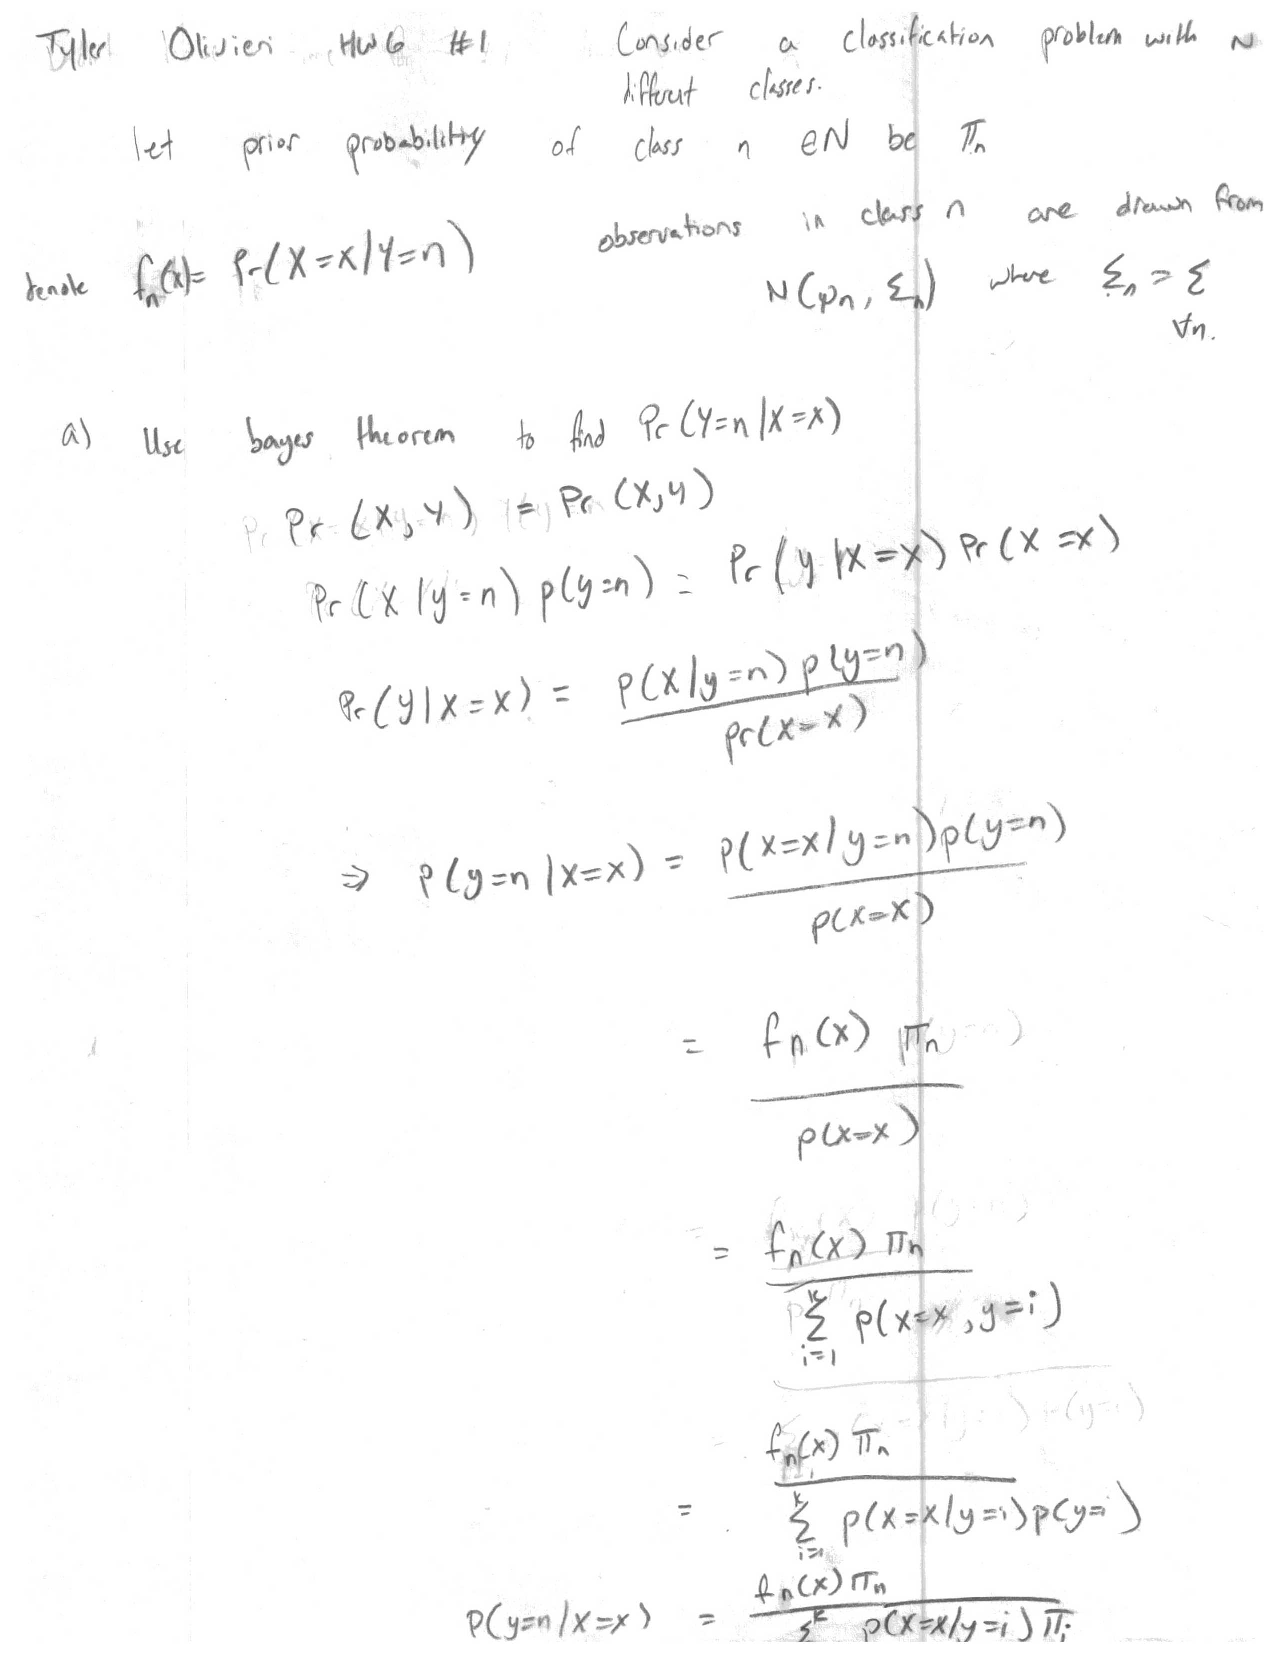
\includepdf[pages=-]{./hw1_3.pdf}  

\item
  Sparse Principal Component Analysis

  \begin{enumerate}
  \item
    The top five components are:
    \begin{enumerate}
    \item
      First component:
      
      [ 0.48788336 -0.26512898  0.47333547  0.13915442  0.19742679 -0.04588071
      0.00406675  0.37030119 -0.43272085  0.25453535 -0.07317678  0.11248878]

      Expained Variance (\%):
      26.009731
     \item
       Second component:
       
        [-0.00417321  0.33896786 -0.1373581   0.16773634  0.18978819  0.25948314
        0.36397137  0.33078079 -0.06544015 -0.10933362 -0.50270865 -0.47316621]

        Expained Variance (\%):
        18.68235

     \item
       Third component:
       
     [-0.16482854 -0.22708884  0.10022856  0.24362014 -0.02660785  0.61611132
   0.54073214 -0.16872267  0.06977056  0.21291324  0.22497138  0.22336929]

   Expained Variance (\%):
   14.024331
   
     \item
       Fourth component:
       
     [-0.23109808  0.04185824 -0.0567358  -0.38303758  0.65477782 -0.03371148
  -0.02845973 -0.20069341 -0.00546618  0.56050237 -0.09170143 -0.03666923]

  Expained Variance (\%):
  10.125174

   \item
     Fifth component:
     
      [-0.07877938  0.29937933 -0.12014871  0.70936319  0.26623723 -0.15941286
      -0.21845284  0.20879298  0.25764682  0.21483493  0.25972635  0.13758414]]

      Expained Variance (\%):
      08.11053
      
    \end{enumerate}
    
  \item

    The scatter plot of data with principal components overlayed:

    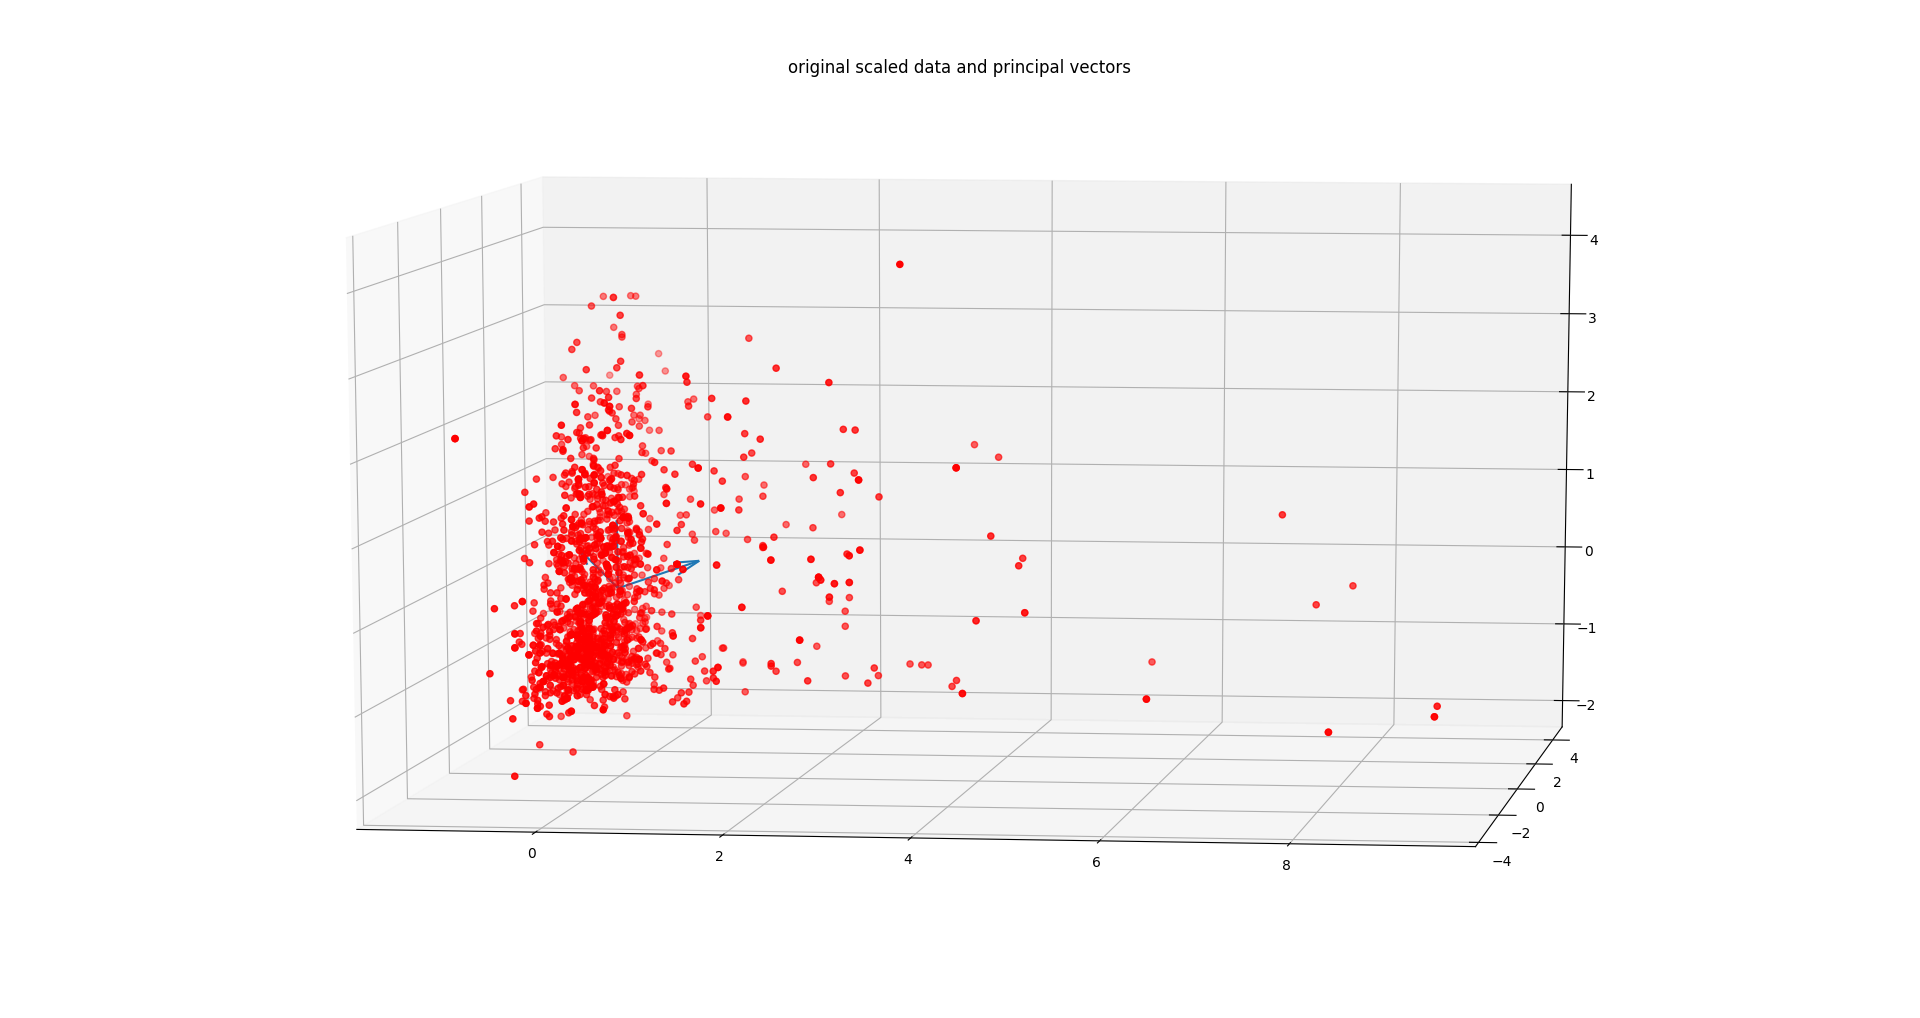
\includegraphics[width=\textwidth]{data_and_pcVectors.png}

    The scatter plot of projected data onto the principal components:

    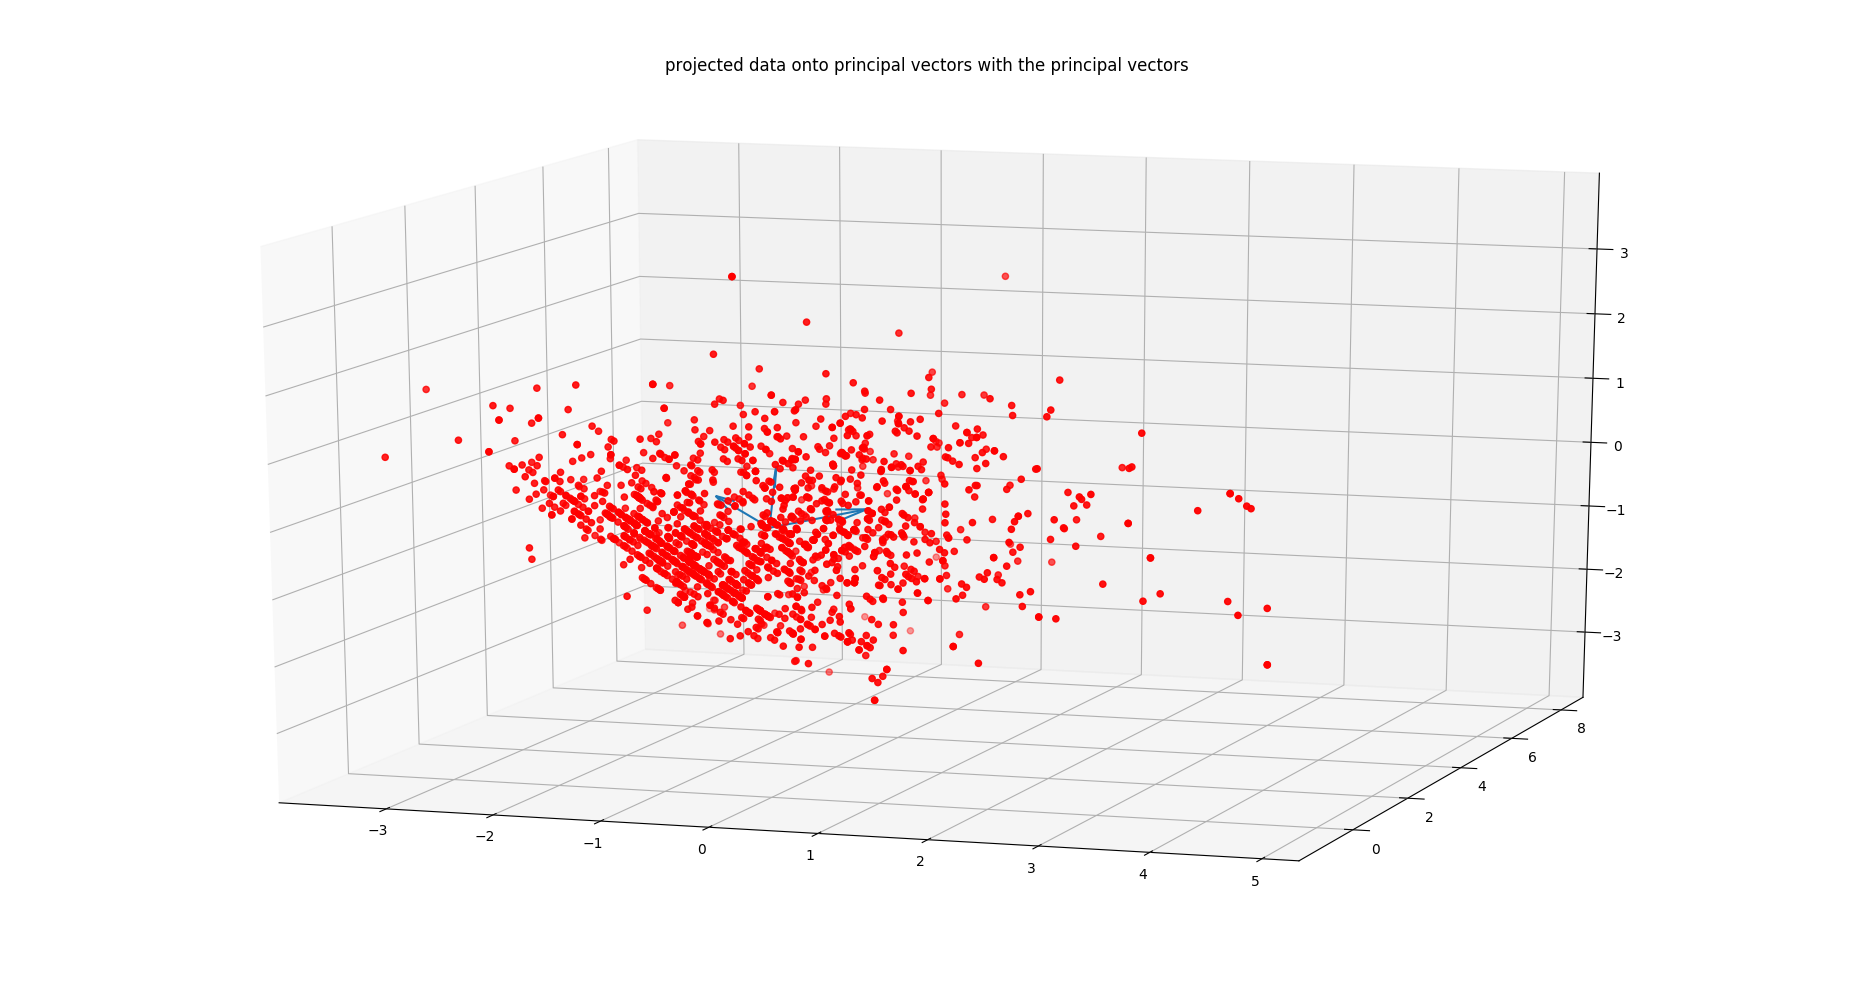
\includegraphics[width=\textwidth]{projected_data_onto_pcVectors.png}
    

  \item

    The $R^2$ value is 0.321.

    The model coefficients are:
    
    x1: 0.0627
    
    x2: -0.2787
    
    x3: 0.3206

    Accordingt to "An Introduction to statistical learning theory in R'', the loadings define the direction in the the feature space along which the data vary the most. These are normalized eigenvectors. We can obtrain these from sklearn pca components attribute.

    [ 0.48931422 -0.23858436  0.46363166  0.14610715  0.21224658 -0.03615752
    0.02357485  0.39535301 -0.43851962  0.24292133 -0.11323206]
    
  [-0.11050274  0.27493048 -0.15179136  0.27208024  0.14805156  0.51356681
  0.56948696  0.23357549  0.00671079 -0.03755392 -0.38618096]
  
 [-0.12330157 -0.44996253  0.23824707  0.10128338 -0.09261383  0.42879287
 0.3224145  -0.33887135  0.05769735  0.27978615  0.47167322]
 

    
  \item
    After using sparse pca, the $R^2$ value is 0.323.

    The model coefficients are:

    x1: -4.6641

    x2: -2.9691

    x3: -21.9510

    The loadings are:

    [-33.87131683  15.72735184 -31.68687504  -8.83849947 -13.74979027
    2.44079956   0.         -26.9239972   30.00435285 -15.78203424
    6.83363042]
    
 [ -6.80249127   0.           0.          14.92471163   1.00922725
   34.92211952  34.79148067   0.           0.35007081   3.41756928
   -1.92414012]
   
 [  0.          26.78666359 -15.35603701   0.           7.4091256
   -3.59452513   0.          18.65177905   0.         -11.59880185
   -30.60466288]
   


    The results are similar, as expected. Both PCA and sparse PCA projected datasets produced a model that could explain about the same amount of variance in the data (we can observe this from the  $R^2$ value). This more or less states that PCA and sparse PCA preserved about the same amount of variance in the original dataset through both transformations.  The different coefficients from the regression suggest that even though about the same amount of variance is preserved, the projected data is different (with respect to the coordinates). Actually observing the projected data from sparse PCA shows many components are 0 (which is the goal), to project into a sparse representation. This can make analyzing high dimensional datasets easier.
    
  \end{enumerate}

  \lstinputlisting[language=Python]{hw6_4.py}  
   
\item
  The eigenfaces for the first 150 components can be seen below. (The png's didnt fit on the page nicely, so this is a lot of pages, I apologize)

  First eigenface:
  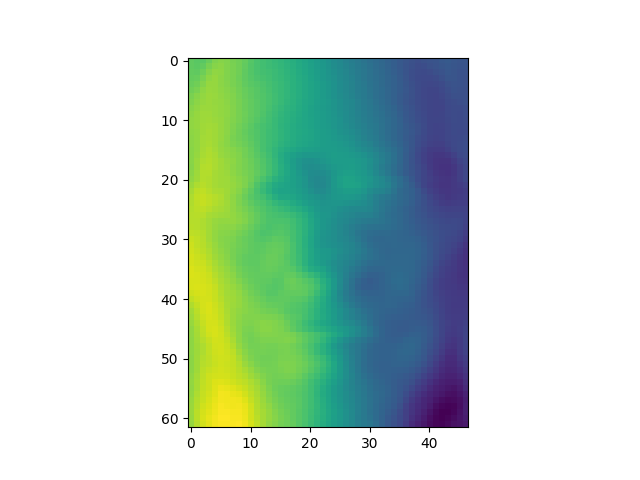
\includegraphics[width=\textwidth]{eigenface_1.png}
  Second:
  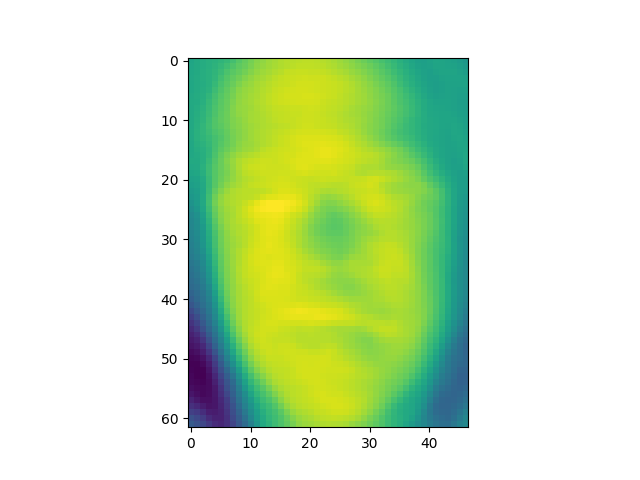
\includegraphics[width=\textwidth]{eigenface_2.png}
  Third:
  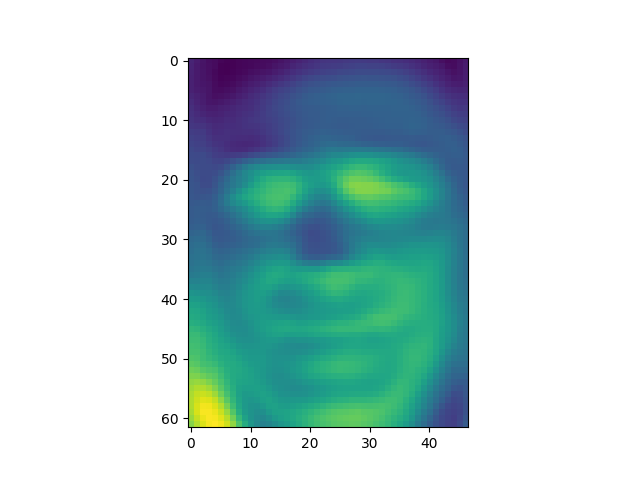
\includegraphics[width=\textwidth]{eigenface_3.png}
  Fourth:
  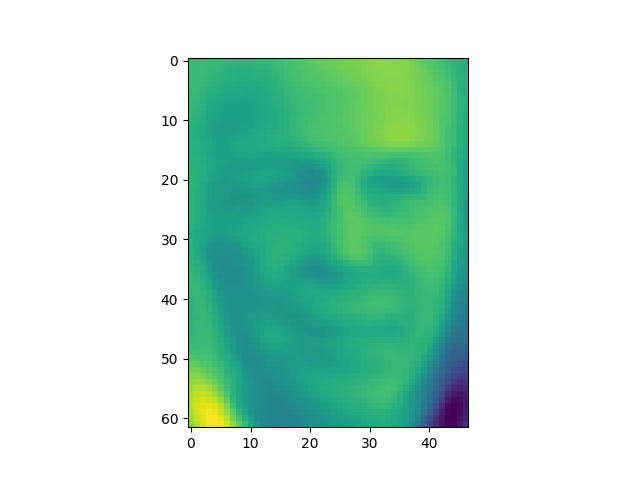
\includegraphics[width=\textwidth]{eigenface_4.png}
  Fifth:
  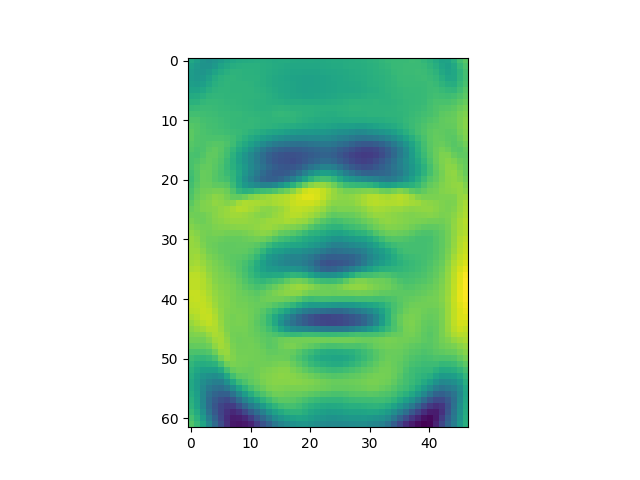
\includegraphics[width=\textwidth]{eigenface_5.png}
  Sixth:
  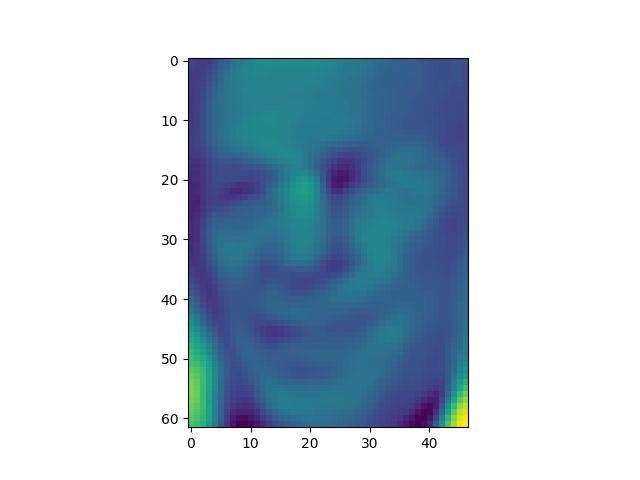
\includegraphics[width=\textwidth]{eigenface_6.png}
  Seventh:
  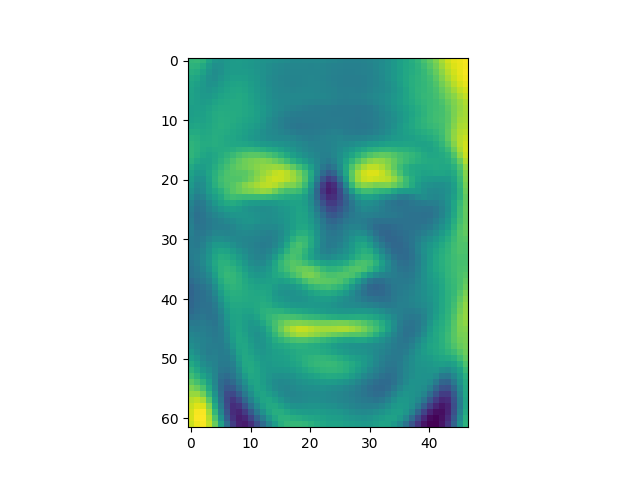
\includegraphics[width=\textwidth]{eigenface_7.png}
  8:
  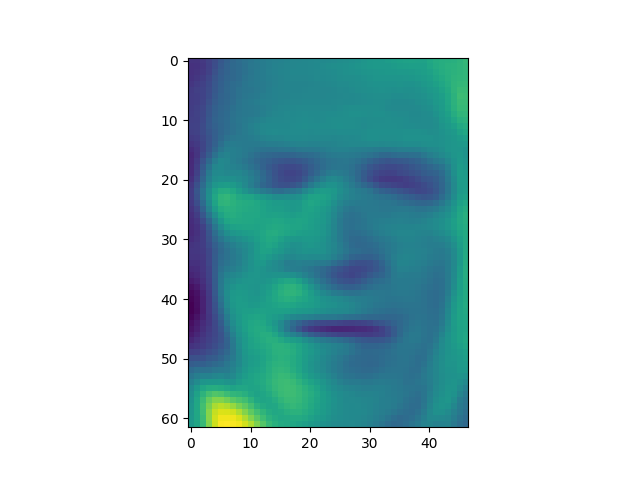
\includegraphics[width=\textwidth]{eigenface_8.png}
  9:
  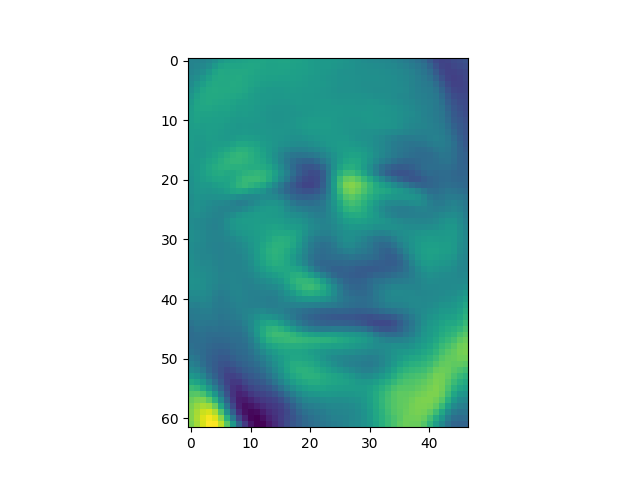
\includegraphics[width=\textwidth]{eigenface_9.png}
  10:
  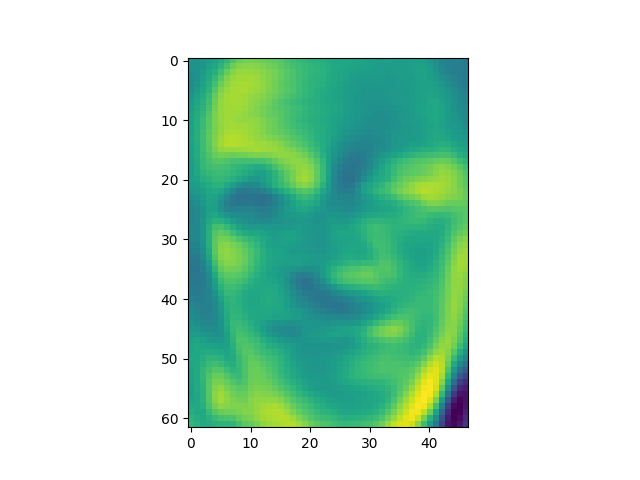
\includegraphics[width=\textwidth]{eigenface_10.png}
  11:
  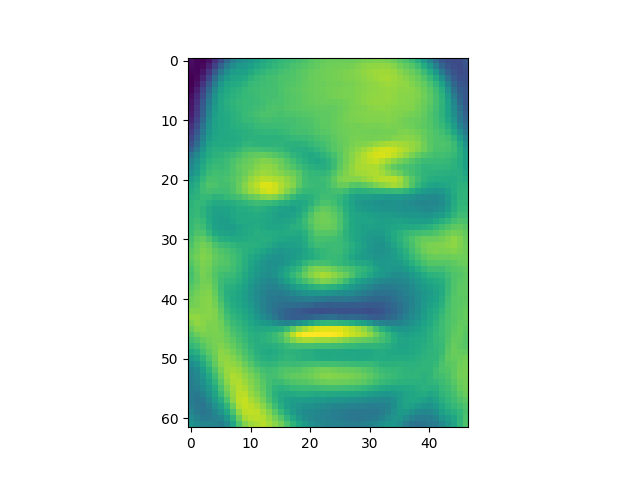
\includegraphics[width=\textwidth]{eigenface_11.png}
  12:
  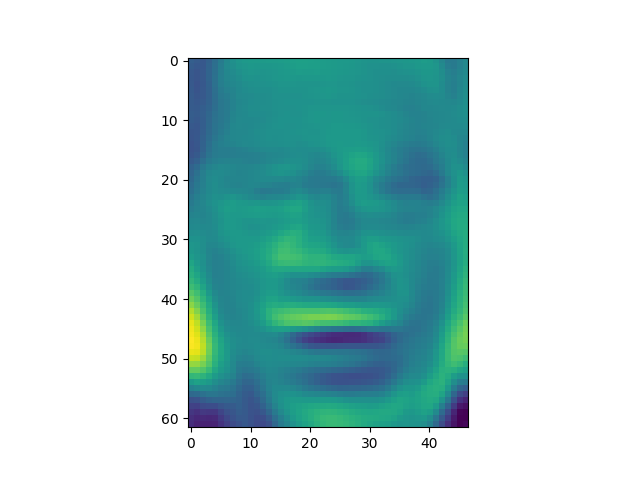
\includegraphics[width=\textwidth]{eigenface_12.png}
  13:
  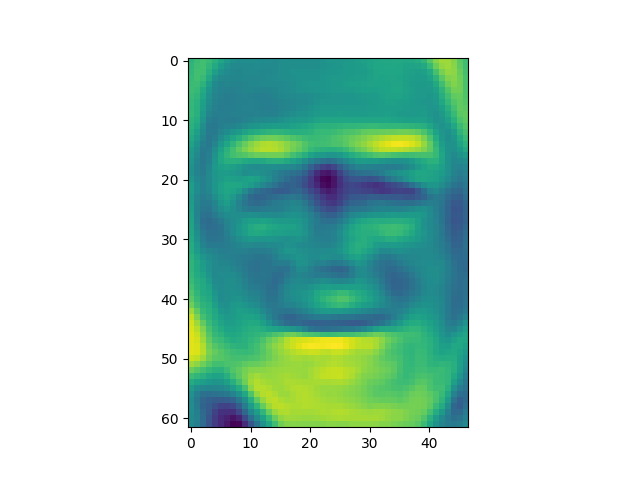
\includegraphics[width=\textwidth]{eigenface_13.png}
  14:
  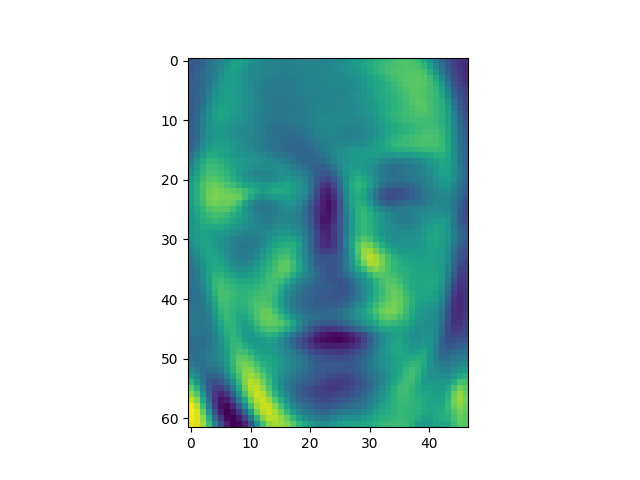
\includegraphics[width=\textwidth]{eigenface_14.png}
  15:
  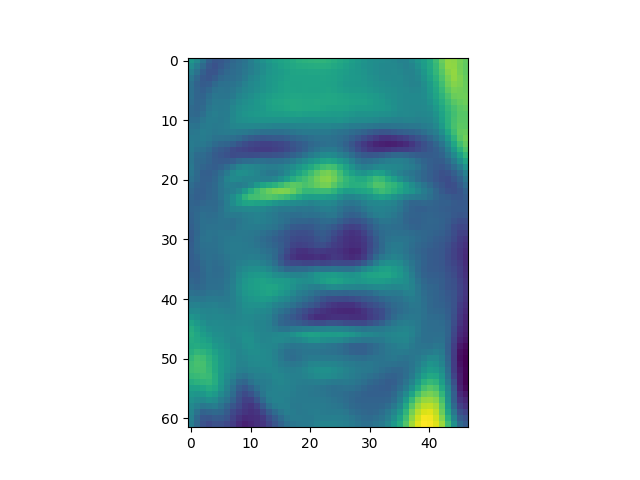
\includegraphics[width=\textwidth]{eigenface_15.png}
  16:
  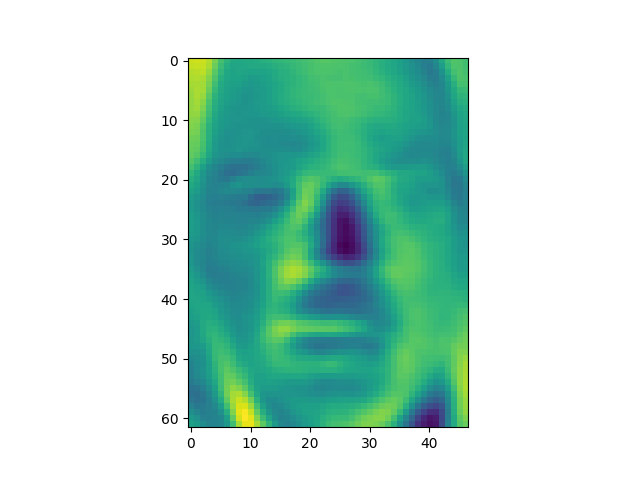
\includegraphics[width=\textwidth]{eigenface_16.png}
  17:
  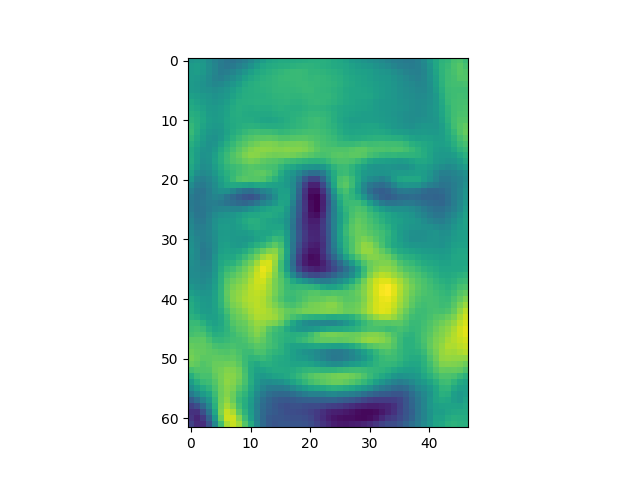
\includegraphics[width=\textwidth]{eigenface_17.png}
  18:
  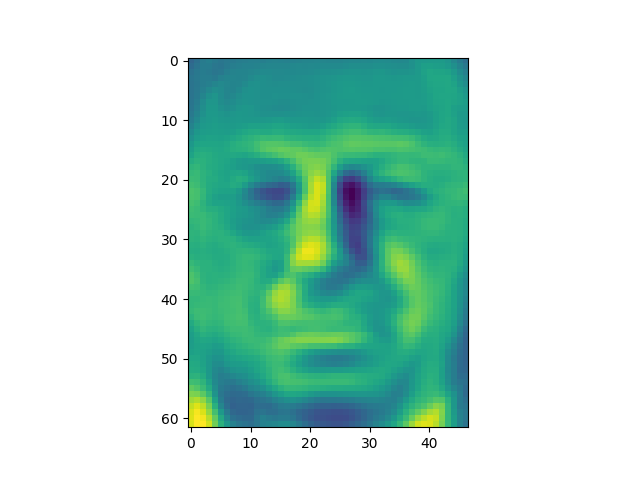
\includegraphics[width=\textwidth]{eigenface_18.png}
  19:
  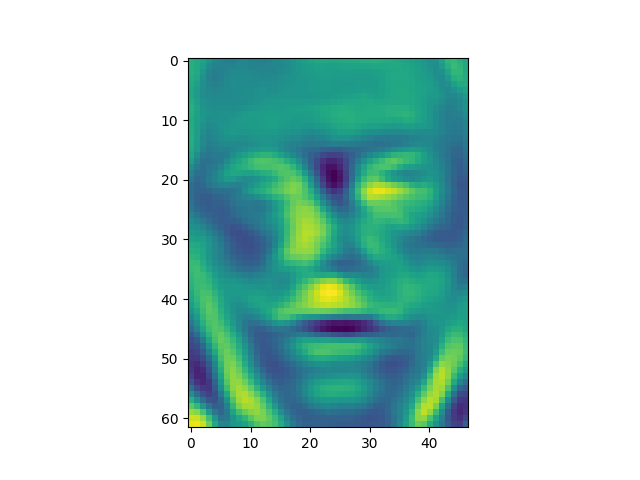
\includegraphics[width=\textwidth]{eigenface_19.png}
  20:
  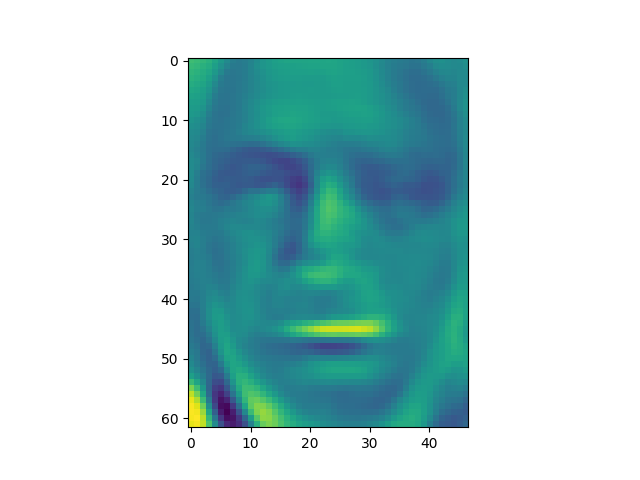
\includegraphics[width=\textwidth]{eigenface_20.png}
  21:
  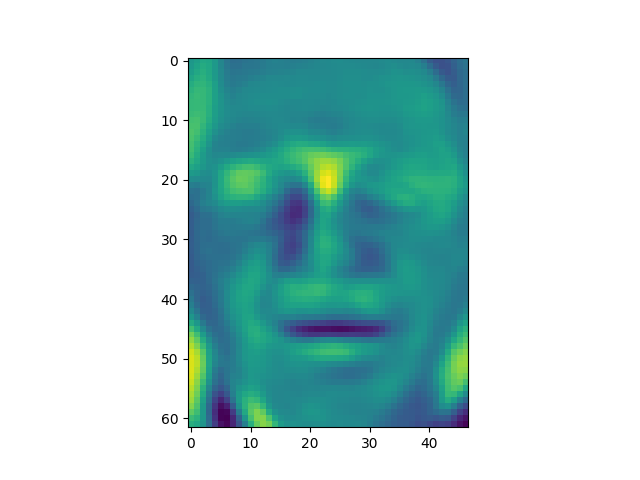
\includegraphics[width=\textwidth]{eigenface_21.png}
  22:
  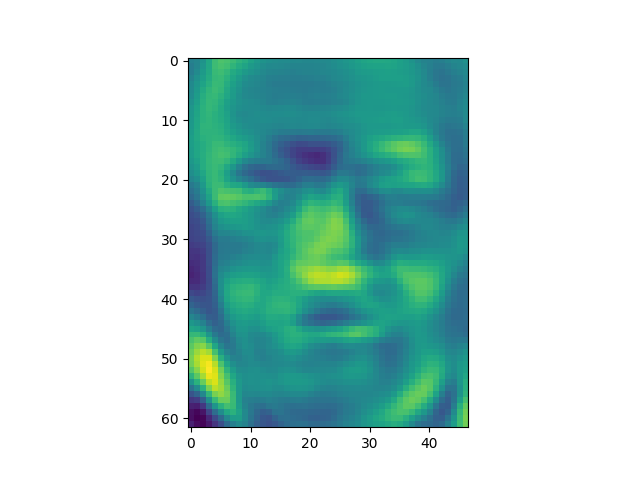
\includegraphics[width=\textwidth]{eigenface_22.png}
  23:
  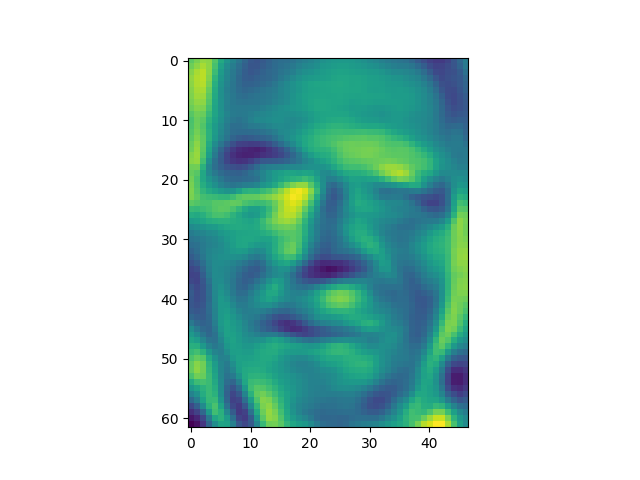
\includegraphics[width=\textwidth]{eigenface_23.png}
  24:
  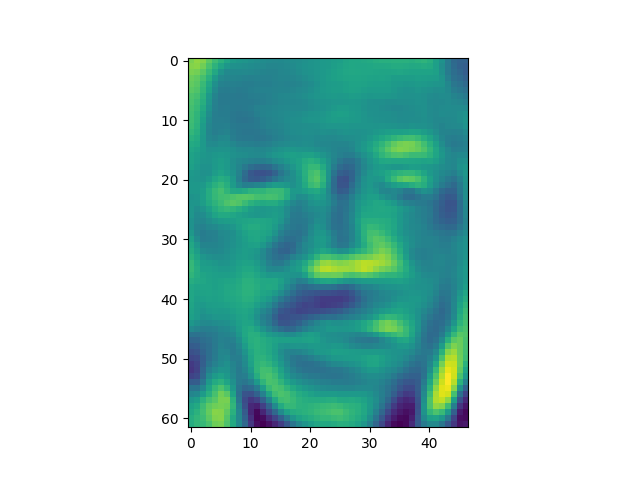
\includegraphics[width=\textwidth]{eigenface_24.png}
  25:
  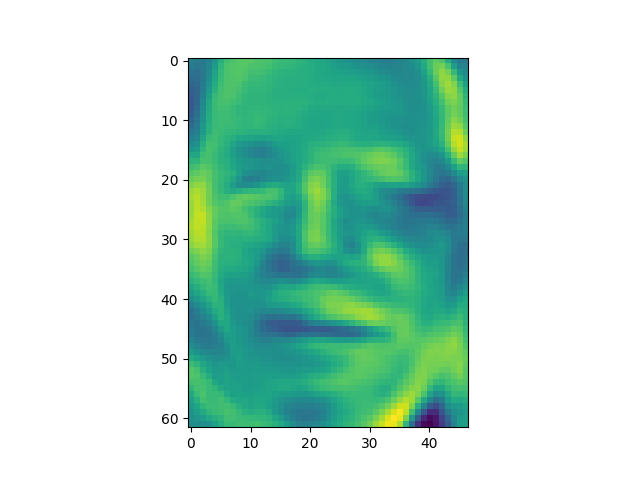
\includegraphics[width=\textwidth]{eigenface_25.png}
  
  A reconstruction of 5 selcted faces:

  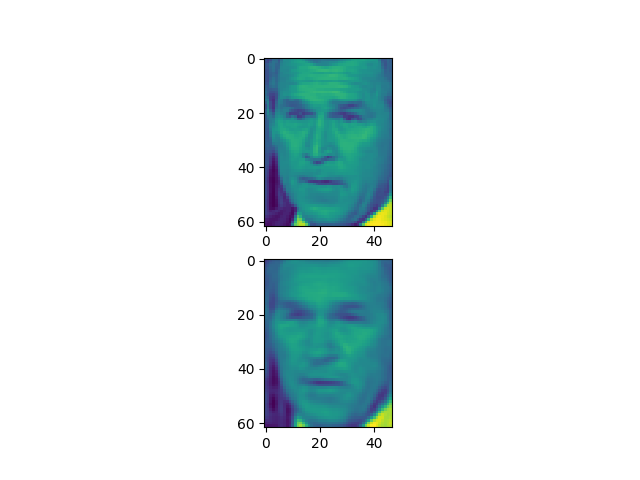
\includegraphics[width=\textwidth]{reconstruct_Im1.png}
  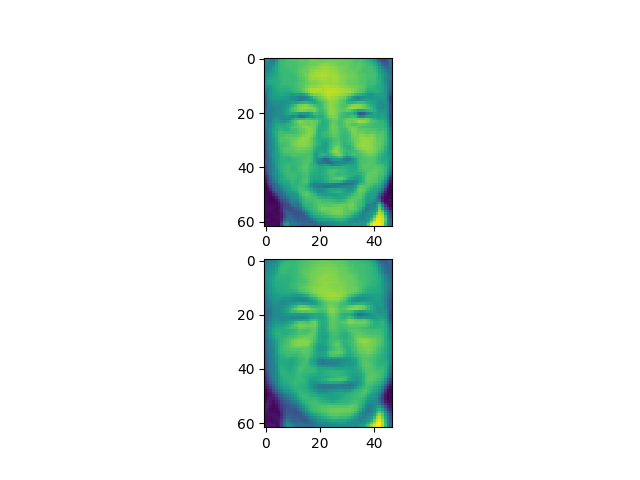
\includegraphics[width=\textwidth]{reconstruct_Im2.png}
  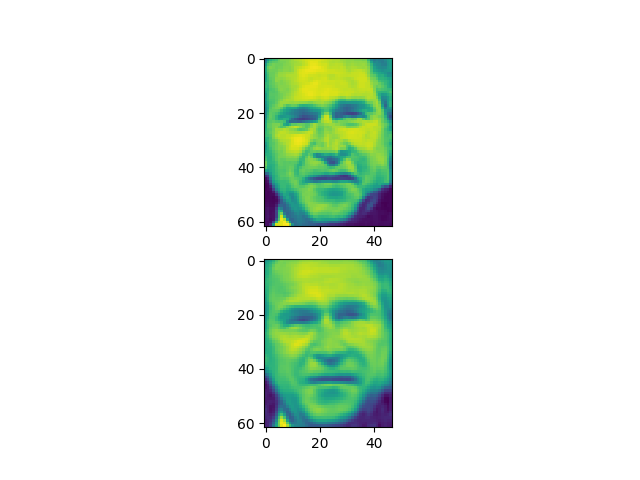
\includegraphics[width=\textwidth]{reconstruct_Im3.png}
  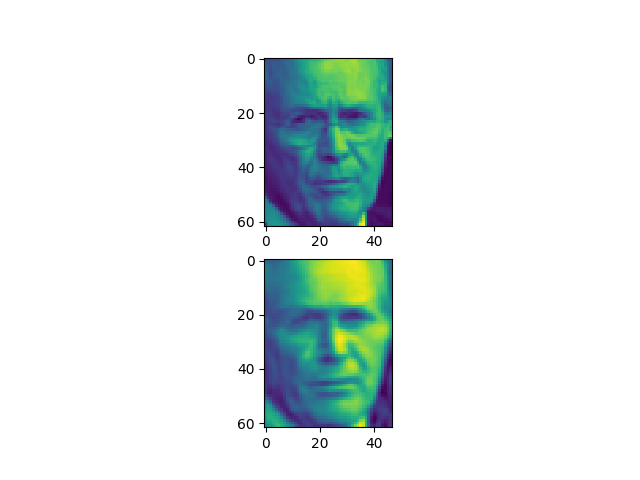
\includegraphics[width=\textwidth]{reconstruct_Im4.png}
  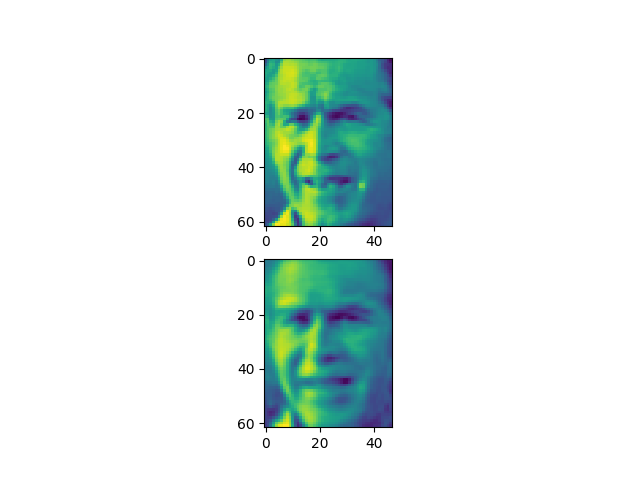
\includegraphics[width=\textwidth]{reconstruct_Im5.png}  

  Python script used to generate the above images:
  \lstinputlisting[language=Python]{hw6_5.py}
  
  
\end{enumerate}

\end{document}

%=========================== END DOCUMENT ==============================

